\documentclass[a4paper,11pt,final]{article}
\usepackage[scaled=0.9]{luximono}
\usepackage[spanish]{babel}
\usepackage[utf8]{inputenc}
\usepackage[T1]{fontenc}
\usepackage{booktabs}
\usepackage{epstopdf}
\usepackage{floatrow}
\usepackage{graphicx}
\usepackage{hyperref}
\usepackage{multicol}
\usepackage{tabularx}
\usepackage{textcomp}
\usepackage{amsmath}
\usepackage{amssymb}
\usepackage{amstext}
\usepackage{caption}
\usepackage{charter}
\usepackage{amsbsy}
\usepackage{amsthm}
\usepackage{lipsum}
\usepackage{minted}
\usepackage{natbib}
\usepackage{array}
\usepackage{color}
\usepackage{esint}
\usepackage{float}

% Hyperref setup
\hypersetup{%
  pdftitle={Procesamiento de datos digitales. Laboratorio 1},
  pdfauthor={César Jiménez Tintaya},
  pdfpagelayout=OneColumn,
  pdfnewwindow=true,
  pdfdisplaydoctitle=true,
  pdfstartview=XYZ,
  plainpages=false,
  unicode=true,
  bookmarksnumbered=true,
  bookmarksopen=true,
  bookmarksopenlevel=3,
  breaklinks=true,
  colorlinks=true,
  linkcolor=blue,
  pdfborder={0 0 0}%
}

% Minted settings
\setminted[matlab]{
  autogobble=true,
  linenos=false,
  bgcolor=grey_lighten_4,
  fontfamily=\ttdefault,
  resetmargins=true,
  stripnl=true,
  breaklines=true
  breakautoindent=true,
  breaksymbolleft=\tiny\ensuremath{\hookrightarrow},
  breaksymbolright=\tiny\ensuremath{\hookleftarrow},
  fontsize=\footnotesize
}

\floatsetup[listing]{
  capposition=top,
  style=plain,
}

\captionsetup[listing]{
  labelfont=bf,
  justification=centering
}

%% LaTeX commands.
\makeatletter
%% -----------------------------------------------------------------------------
% Defining string as labels of certain blocks.
\newcommand{\suma}{\Large$+$}
\newcommand{\inte}{$\displaystyle \int$}
\newcommand{\derv}{\huge$\frac{d}{dt}$}

\definecolor{grey_lighten_4}{rgb}{0.9804, 0.9804, 0.9804}

%% Redefinition of \maketitle command
\def\@maketitle{%
  \newpage
  \null
  \begin{center}%
    \small{\uppercase{Univerisad Nacional Mayor de San Marcos}} \par%
    \vskip 0.5em%
    \small{\uppercase{Facultad de Ciencias Físicas}} \par%
    \vskip 2em%
    \let \footnote \thanks
    \small{\textsc{Procesamiento de Datos Digitales}} \par%
    \vskip 0.5em%
    {\LARGE \@title \par}%
    \vskip 1.5em%
    {%
      \normalsize
      \lineskip .5em%
      \begin{tabular}[t]{c}%
      \@author
      \end{tabular}\par%
    }%
    \vskip 1em%
    {\normalsize \@date}%
  \end{center}%
  \par%
  \vskip 1.5em%
}

\makeatother

%% -----------------------------------------------------------------------------
\begin{document}
  \title{Laboratorio Nº4}
  \author{Lic. César Jiménez Tintaya\\ \small{\texttt{cjimenezt@unmsm.edu.pe}}}
  \date{}
  \maketitle

  \begin{enumerate}
    \item Graficar en \textsc{Matlab} las señales a y b, y hallar
      la transformada de Fourier en forma analítica (usar propiedades):

      \begin{enumerate}
        \item $f_1\left(t\right) = G\left(\frac{t}{2}\right) - G\left(t\right)$
        \item $f_2\left(t\right) = 5G\left(t-1\right) - G\left(t+1\right)$
        \item $f_3\left(t\right)$
          \vspace{-1.5em}
          \begin{figure}[H]
            \begin{center}
              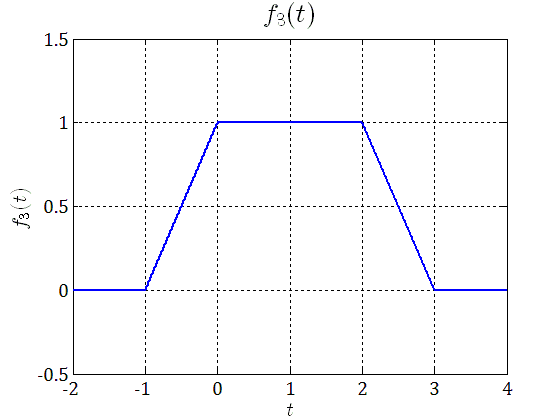
\includegraphics[width=0.5\textwidth]{./lab4prob1c.png}
            \end{center}
          \end{figure}\vspace{-2.5em}

        \item $f_4\left(t\right)$
          \vspace{-1.5em}
          \begin{figure}[H]
            \begin{center}
              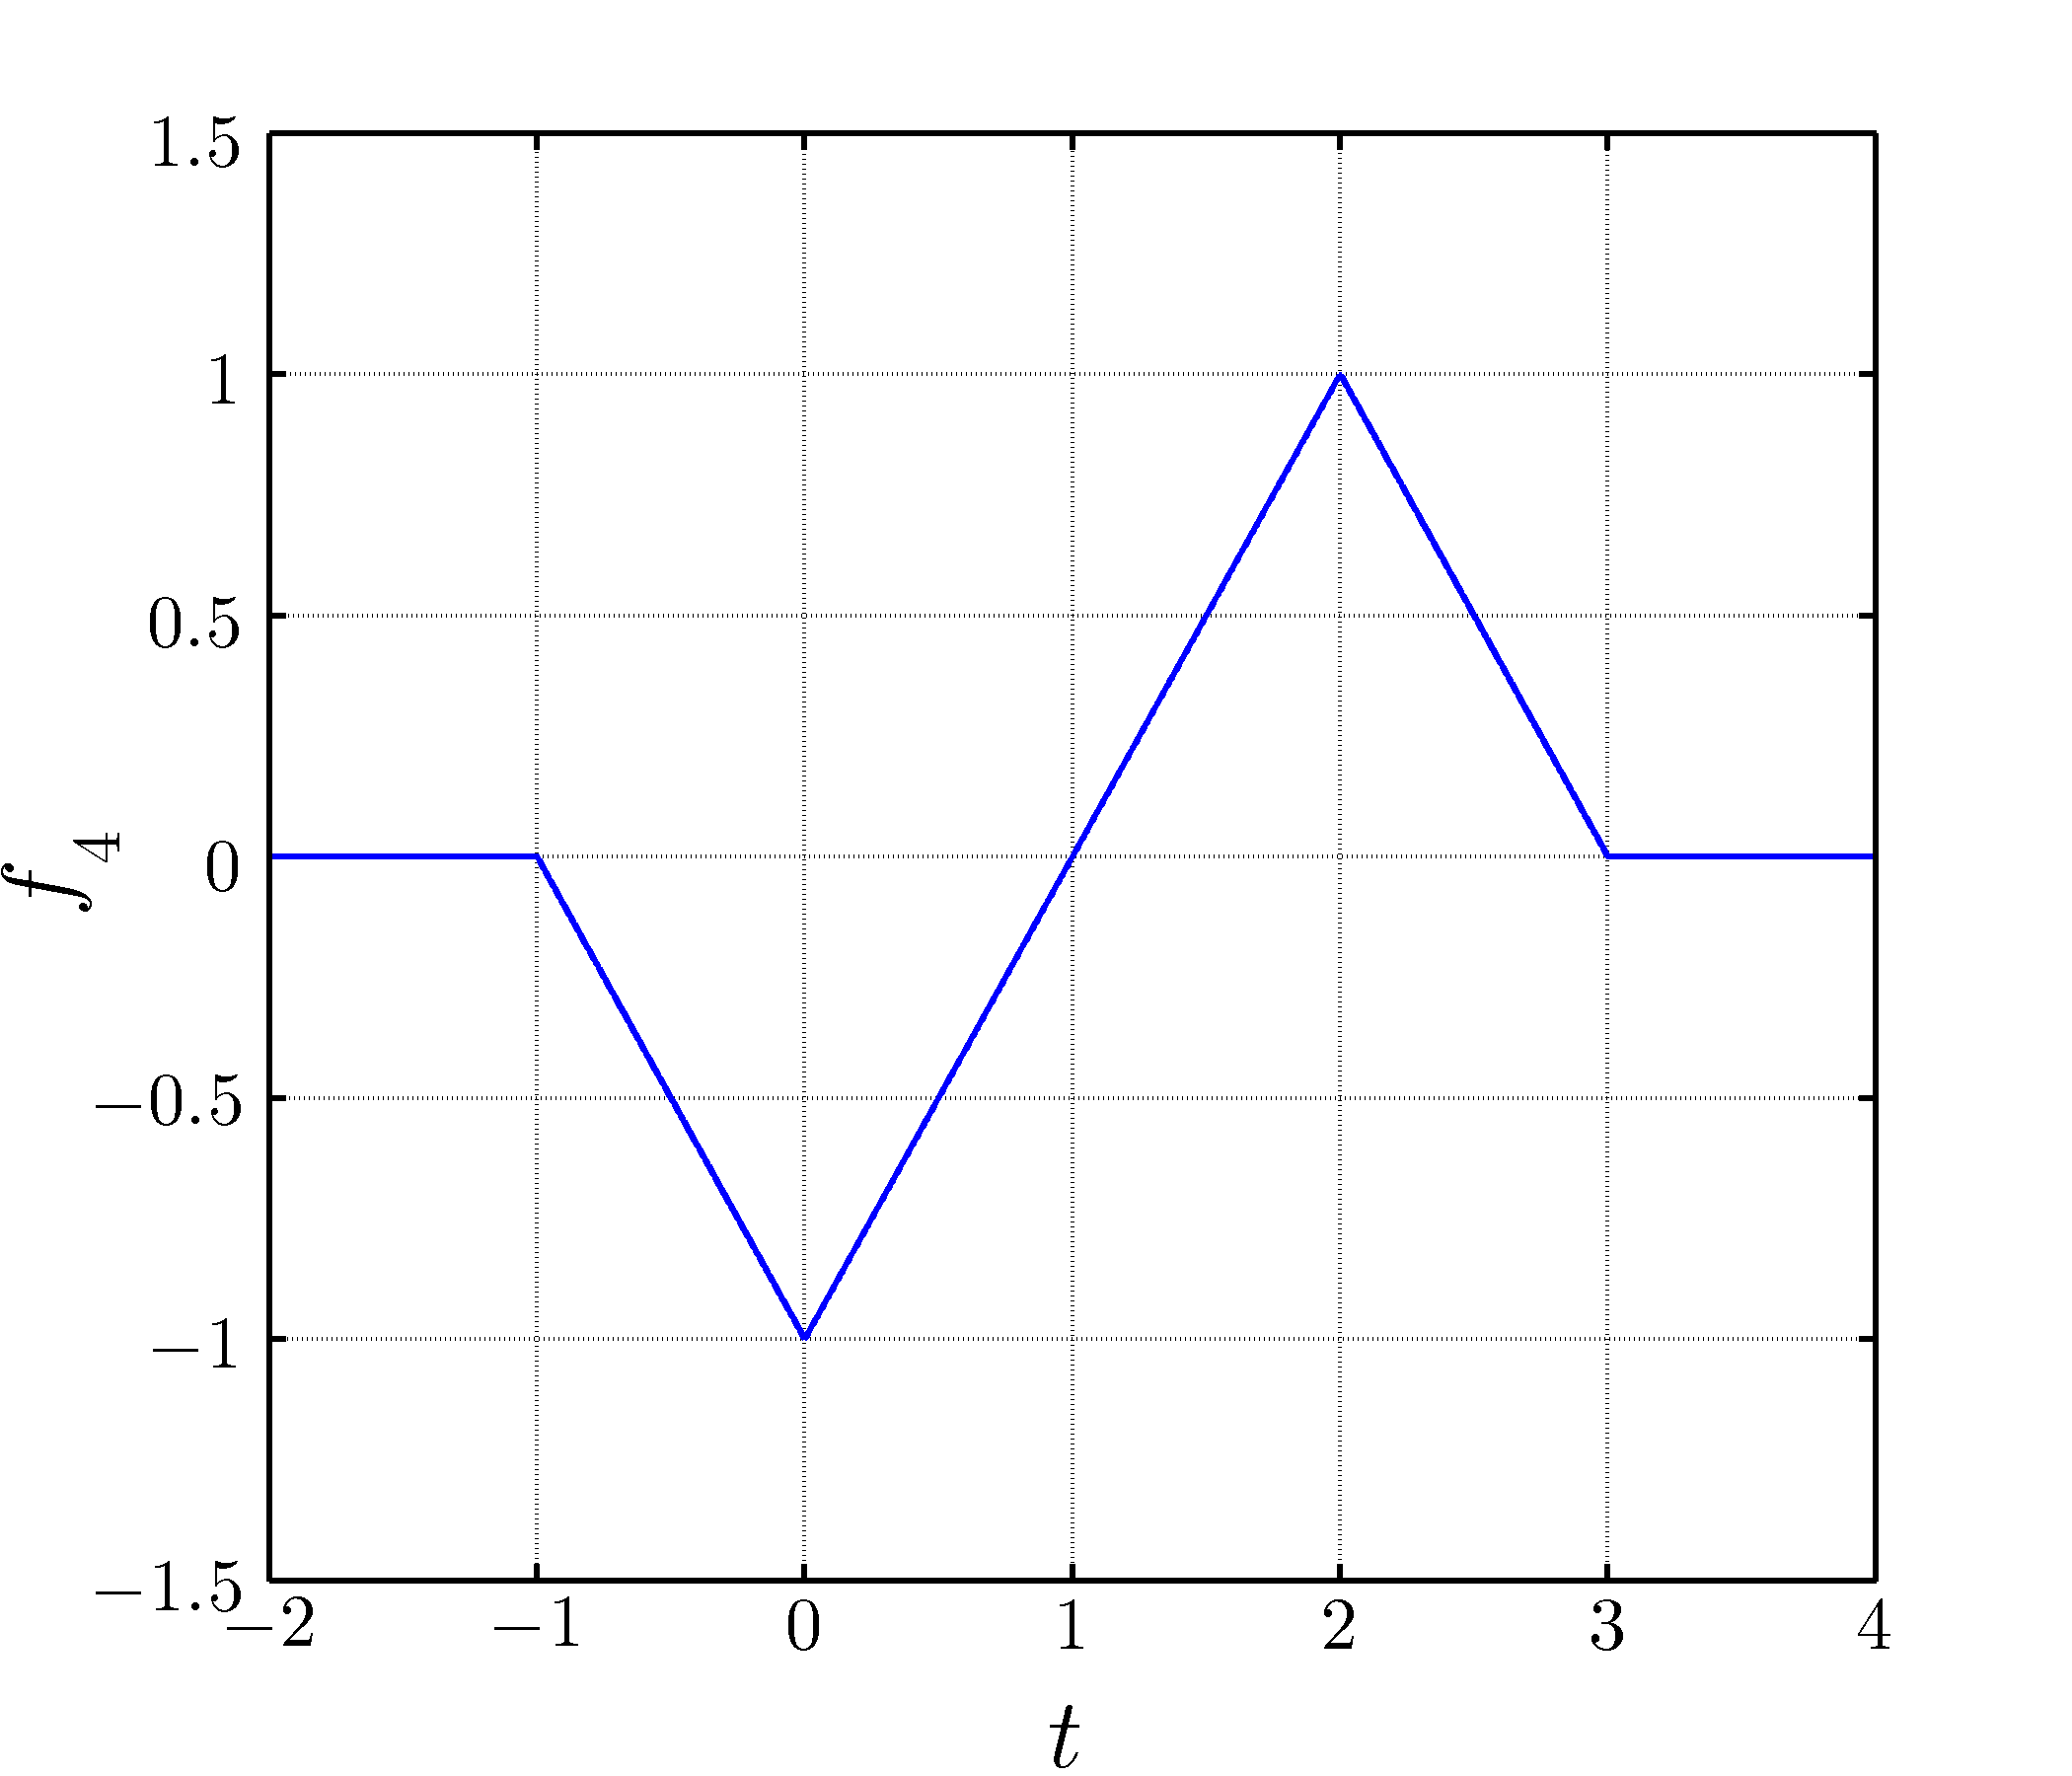
\includegraphics[width=0.5\textwidth]{./lab4prob1d.png}
            \end{center}
          \end{figure}\vspace{-2.5em}
      \end{enumerate}

      \noindent \emph{Nota}: $G$ es la función compuerta unitaria.

    \item Hallar la transformada de Fourier de $x\left(t\right)$ y graficar en Matlab:

      \begin{figure}[H]
        \begin{center}
          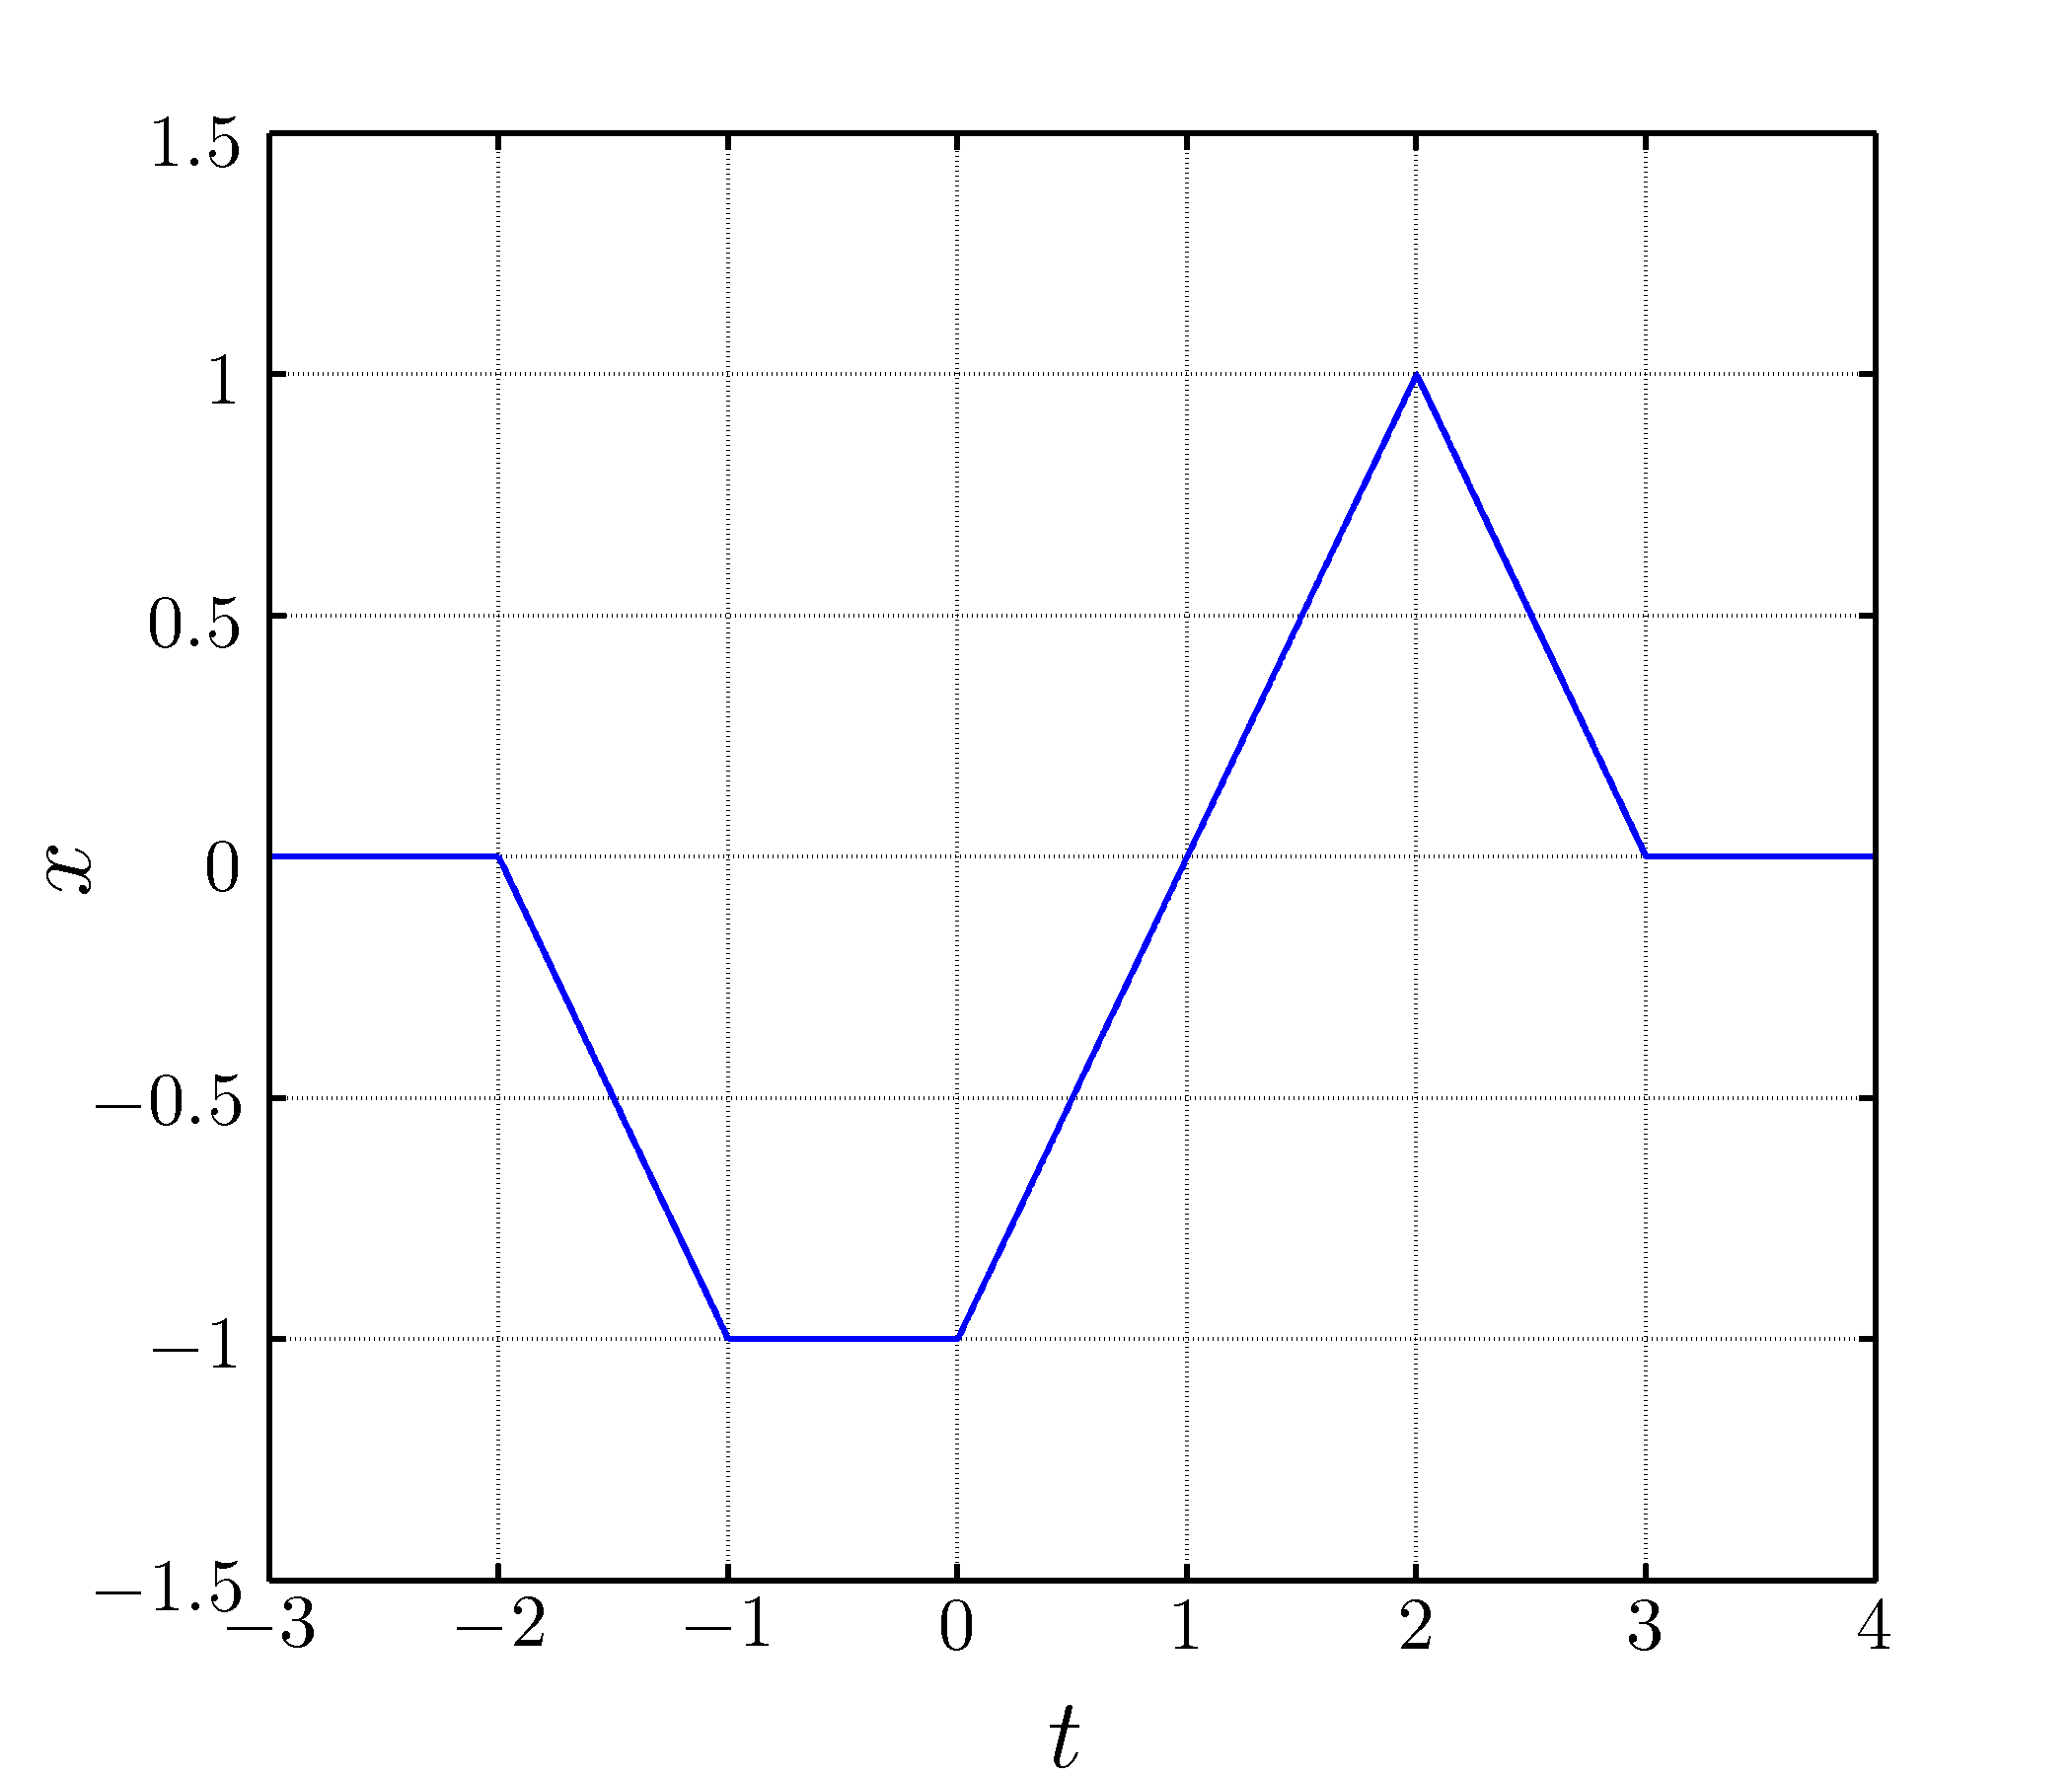
\includegraphics[width=0.5\textwidth]{./lab4prob2a.png}
        \end{center}
      \end{figure}\vspace{-1.5em}

      Si $x\left(t\right)$ pasa a través del bloque de la figura,
      calcule la transformada de Fourier de $y\left(t\right)$.

      \begin{figure}[H]
        \begin{center}
          
\includegraphics[width=0.5\textwidth]{./lab4prob2b.png}
        \end{center}
      \end{figure}\vspace{-1.5em}

    \item Halle y grafique la transformada de Fourier de las siguientes señales:
      \begin{enumerate}
        \item $x\left(t\right)$

          \begin{figure}[H]
            \begin{center}
              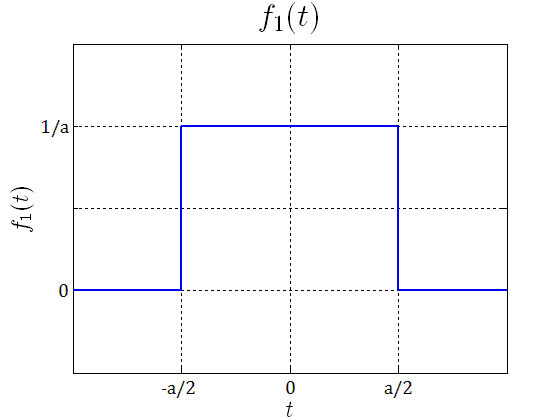
\includegraphics[width=0.5\textwidth]{./lab4prob3a.png}
            \end{center}
          \end{figure}\vspace{-1.5em}

        \item La función periódica mostrada en la figura:

          \begin{equation*}
            x\left(n\right) = \left\{
              \begin{array}{ccl}
                1 & ; & \mathrm{Si}\ n\ \mathrm{impar}\\
                2 & ; & \mathrm{Si}\ n\ \mathrm{par}\\
              \end{array}
            \right.
          \end{equation*}

          con $n \in \mathbb{Z}$.

          \begin{figure}[H]
            \begin{center}
              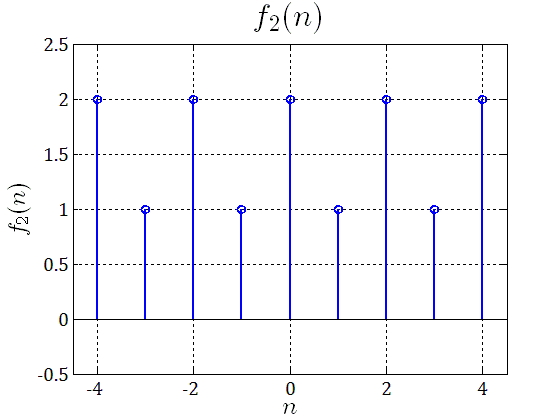
\includegraphics[width=0.5\textwidth]{./lab4prob3b.png}
            \end{center}
          \end{figure}\vspace{-1.5em}

        \item $$f\left(t\right) = t^2\exp\left(-\frac{t}{\tau}\right)$$
      \end{enumerate}
    \item Dada la señal en el dominio del tiempo:

      $$y\left(t\right) = \sin\left(t\right) + 0.25\sin\left(10t\right)$$

      \begin{enumerate}
        \item Hacer un programa para graficar la señal para $4$ periodos, con una frecuencia de muestreo de $100\ Hz$.
        \item Hacer un programa para graficar el espectro de frecuencias de la señal.
        \item ¿Cuál es la amplitud y la frecuencia correspondiente a cada pico?
      \end{enumerate}

    \item Descargue el archivo \texttt{datos.txt}\footnote{\url{http://fenlab.9k.com/pds/datos.rar}} de la web, que representa una señal de audio.
      La frecuencia de muestreo es de $F_s = 8000\ Hz$. Hacer un programa en Matlab para que realice
      lo siguiente:

      \begin{enumerate}
        \item Hallar el número de datos N.
        \item Hallar la duración de la señal.
        \item Hallar el valor medio de la señal.
        \item Graficar la señal $x\left(t\right)$.
        \item Graficar el espectro de frecuencias.
      \end{enumerate}

    \item En matlab realizar lo siguiente
      \begin{enumerate}
        \item Calcule y grafique la transformada de Fourier de la función triángulo:
              $$x\left(t\right) = \Lambda\left(\frac{t}{2}\right)$$
        \item La integral que define la transformada de Fourier puede calcularse
          numéricamente, para cada valor de frecuencia, utilizando la suma de
          Riemman. Para subdominios de longitud T se tiene:

          $$X\left(f\right)=\sum_{N=-\infty}^{\infty}\Lambda\left(\frac{n T}{2}\right)\exp(-2\pi j f N T )T$$

          Calcular para $T=0.8$ y para el rango de frecuencia de $0$ a $2$ con
          intervalos de $0.125$ ejecutando las siguientes sentencias en Matlab:

          \begin{listing}[H]
            \setbox0=\vbox{%
              \begin{flushright}
                \begin{minipage}[t]{\textwidth - 50pt}
                  \begin{minted}{matlab}
                    T = 0.8;
                    n = [-2:2];
                    f = [0:0.125:2];
                    X = zeros(size(f)) ;
                    for i = 1: length(f)
                        X(i) = sum(T*triang(n*T/2).*exp(-j*2*pi*f(i)*n*T);
                    end
                  \end{minted}
                \end{minipage}
              \end{flushright}
            }%
            \makebox[\textwidth][l]{\box0}
          \end{listing}\vspace{-1.5em}

        \item Repetir para $T$ $10$ veces menor.
      \end{enumerate}

      \emph{Nota}: La función $\Lambda$ es la función triángulo
      $\Lambda\left(t\right)$ que Ud. debe implementar en \textsc{Matlab}.
  \end{enumerate}
\end{document}

